\documentclass[12pt]{article}

\usepackage{fullpage}
\usepackage{times}
\usepackage{url}

\usepackage{rosetta}
\usepackage{graphicx}
%\usepackage{diagrams}
\usepackage{comment}


\bibliographystyle{unsrt}

\begin{document}

\noindent
{\Large Title: \textbf{Heterogeneous Modeling using a Lattice of Coalgebras}}

\bigskip
\bigskip
\bigskip
\bigskip
\bigskip

\noindent
Technical Area: \textbf{TA2}

\bigskip
\bigskip
\bigskip
\bigskip

\noindent
Organizations: \begin{minipage}[t]{4in}
  \textsf{University of Cincinnati} \\
  \textsf{University of Kansas} \\
  \textsf{University of California @ Riverside}
\end{minipage}

\bigskip
\bigskip
\bigskip
\bigskip

\noindent
Technical Point of Contact: \begin{minipage}[t]{4in}
  Philip A. Wilsey \\
  Dept of EECS, PO Box 210030 \\
  Cincinnati, OH 45221--0030 \\
  (513) 556--4779 (voice) \\
  (513) 556--7326 (fax) \\
  \url{philip.wilsey@uc.edu}
\end{minipage}

\clearpage

\section{Introduction}

This document addresses \textbf{TA2} and presents ideas for the multi-resolution modeling
of complex heterogeneous networked multi-scale systems-of-systems (SoS).  The proposed
approach uses a \emph{Lattice of Coalgebras} to provide a framework that enables the
design and quantitative assessments of SoS systems.  The use of a Lattice of Coalgebras
promotes the ability to bring together heterogeneous multi-domain models into a common
framework to access the impact of local decisions on global properties.  By using a
lattice-based approach we can use Galois connections and functors to develop \emph{safe}
transformations between disparate domains.  These safe transforms then allow the alignment
of multi-domain system models into a unifying SoS model for analysis.  Furthermore, we
propose using coalgebras (over algebras) due to the non-terminating and heterogeneous
nature of SoS.  Coalgebras are more natural than algebras for representing non-terminating
systems.  The inductive proof theory associated with algebras requires a base case or
initial state that may not exist in many embedded systems.  As stream transformers,
coalgebras and their associated proof techniques are well equipped to deal with reactive,
non-terminating embedded systems.

\subsection{A Lattice of Domains}

Vocabulary and semantics for defining models in a specific domain can be thought of as a
\emph{modeling domain} or simply \emph{domain}.  Each domain provides to varying degrees
units of semantic representation, (i) a model of computation, and (ii) a domain specific
modeling vocabulary.  Ideally, a domain defines a collection of definitions that
characterize a particular computation or modeling style.

When a new model is written, it \emph{extends} a domain using that domain as a semantic
basis an to define vocabulary.  In this way, the domain defines the type of a model.  For
example, if a simulator is defined of type \lstinline!state_based!, then the concepts of
state, change and event are available as a built-in part of the specification vocabulary.

When a new modeling domain is defined, it is typically a subdomain of some existing
modeling domain.  Like a model, the new domain extends the original domain and inherits
all of that domain's declarations.  For example, if a new \lstinline!discrete_time! domain
is defined as a subtype of \lstinline!state_based!, then the notions state and change are
inherited and refined within the new domain.

Modeling domains and their associated extensions define a lattice we will refer to as a
\emph{domain lattice}.  The set of domains, $D$, together with the homomorphism
relationships resulting from extension define a partially ordered set $(D,\Rightarrow)$.
Join ($\sqcup$) and meet ($\sqcap$) can subsequently be defined as the least common
supertype and greatest common subtype of any pair of domains.  It can easily be proved
that any domain pair will in fact have a least common supertype and a greatest common
subtype.  The \lstinline!null! domain is the least domain in the collection and all
domains inherit from it.  \lstinline!bottom! is the greatest domain and inherits from all
domains making it inconsistent.  Specifically:

\[\forall m:model \cdot \mathsf{bottom} \Rightarrow m \wedge m \Rightarrow \mathsf{null}\]

\noindent
Including \lstinline!null! and \lstinline!bottom! with the partially ordered set
$(D,\Rightarrow)$ defines a lattice whose top and bottom elements are \lstinline!null! and
\lstinline!bottom! respectively:

\[(D,\Rightarrow,\sqcup,\sqcap,\mathsf{null},\mathsf{bottom})\]

\subsection{Coalgebraic Semantics}

The semantics of both domains and models is denoted by a
coalgebra~\cite{Jacobs:97:A-Tutorial-on-C} defining observations on an abstract state,
$\abstate$.  The signature for a coalgebra is:

\[\langle x,y,z,s \rangle::\abstate \rightarrow
T_x\times T_y\times T_z\times T_s\]

%% PERRY: how do we (quickly) tie in or remove Rosetta from this document??  i have no
%% strong thoughts either way, but we will lose time introducting Rosetta and wonder if
%% it's best to use an abstracting functor to remove it for this whitepaper; focusing on
%% the lattice and coalgebra theory fundamentals....rather than screw it up; i'll let you
%% execute this functor (i don't know if i should thank you or curse you for this stuff,
%% but it's been a fun couple of days....and some of it is beginning to make sense).

\noindent where $x$, $y$, $z$, and $s$ are observations on $\abstate$
and $T_x$ through $T_s$ are the types of those observations.  When $s$
is treated as state, this signature has the form of a classic
coalgebraic model.  For any observation, $x$, made relative to state,
the associated type will be $T_s\rightarrow T_x$, a functional mapping
from a state value to a value of the type associated with the
observation.  One particularly important observation is the next state
given by \lstinline!next(s)! of type $T_s\rightarrow T_s$ mapping one
system state observation to another.

%% We choose coalgebras over their better known duals, algebras, due to the
%% non-terminating and heterogeneous nature of the types of systems we model.  Coalgebras
%% are more natural than algebras for representing non-terminating systems.  The inductive
%% proof theory associated with algebras requires a base case or initial state that may
%% not exist in many embedded systems.  As stream transformers, coalgebras and their
%% associated proof techniques are well equipped to deal with reactive, non-terminating
%% embedded systems. 

The heterogeneous nature of system-level specifications requires that multiple computation
models be considered during modeling and analysis.  In the coalgebra, $\abstate$ can be
held abstract with no associated concrete type.  Specific states simply become
observations of the abstract state making multiple simultaneous state observations
possible.  Furthermore, by defining relationships between states in different domains, one
can relate information associated with one state observation to information associated
with other state observations.  This critical feature allows determination of when
information observed in one domain impacts information observed in another.

\section{Lattice of Coalgebras}

Using this semantic basis, we can use the domain lattice to define specification
transformation and composition.  Additionally, the lattice facilitates establishing the
safety of such operations using Galois connections.  Each of these is critical to
supporting model heterogeneity and composition necessary for system-level design.

% Functors and products discussed in this section and homomorphisms
% discussed earlier are examples of reflective Rosetta operations making
% up the \emph{facet algebra} used to compose specifications.  Products
% compose specifications and functors transform specifications to define
% new specifications. Homomorphism is a relation over specification
% pairs.  Other important facet algebra operations include equivalence
% (isomorphism), relabeling and instantiation.

%% PERRY: if we remove the discussion of Rosetta from the document, we can still use this
%% graphic, just without the qualification of it as a Rosetta Domain Lattice, we could
%% simply label it as an Example Domain Lattice; i believe the terms used in it are
%% reasonably standard to someone with a computing background so as to be understood
%% without a language basis....

\begin{figure}[hbtp]
  \centering
  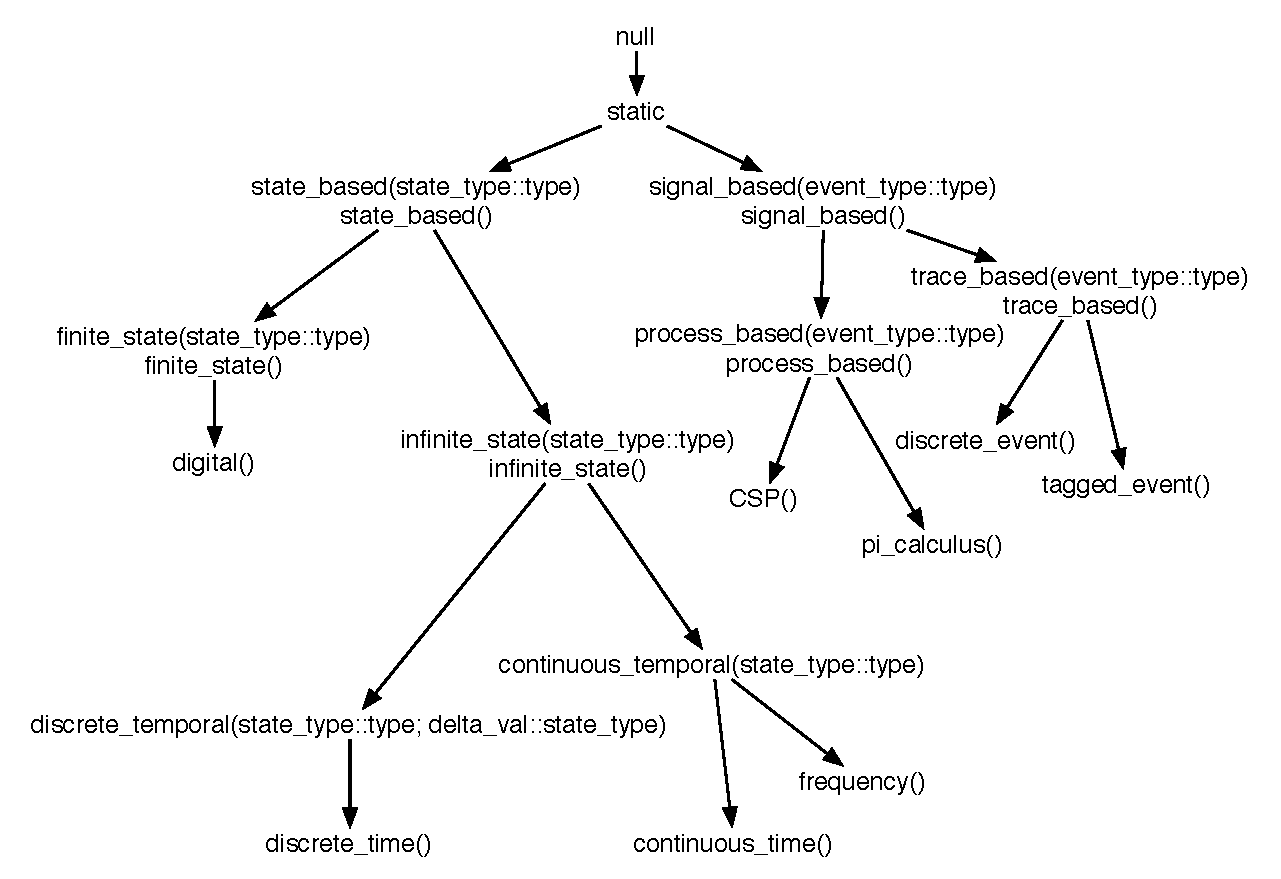
\includegraphics[width=0.6\textwidth]{figures/semi-lattice-detailed.pdf}
  \caption{Example modeling domain Lattice}
  \label{fig:semi-lattice-detailed}
\end{figure}

\subsection{Functors and Specification Transformation}

A \emph{functor} in the domain lattice is a function specifying a
mapping from one domain to another.  The primary role of functors in
the domain lattice is to transform a model in one domain into a model
in another.  Viewing each domain and facets comprising its type as a
subcategory of the category of all models, a functor is simply a
mapping from one subcategory to another.  Any model in the original
category can be transformed into a model in the second.  This
corresponds to the classic definition of functors in category theory.

When defining domains by extension, two kinds of functors result.
Instances of concretization functors, $\Gamma$, are defined each time
one domain is extended to define another.  Abstraction functions, $A$,
are the dual of concretization functions and are known to exist for
each $\Gamma$ due to the multiplicative nature of extension.  $\Gamma$
instances move down in abstraction while $A$ instances move up.  Each
extension between domains defines both an instance of $\Gamma$ and
$A$.  However, $A$ and $\Gamma$ do not form an isomorphism because $A$
is lossy -- some information must be lost or $A$ cannot truly be an
abstraction function.

\subsection{Safety and Galois Connections}

Abstract interpretation~\cite{Cousot:00:Abstract-Interp} provides a
capability for focusing analysis by eliminating unneeded detail from a
specification.  Among the most challenging problems in abstract
interpretation is assuring that once the abstraction is performed the
resulting model is faithful to the original. This is the notion of
\emph{safety} -- assuring that when an abstraction is performed, the
information retained is correct.  Establishing a \emph{Galois
  connection} \cite{Nielson:05:Principles-of-P} between domains in the
lattice provides exactly this assurance.

A Galois connection ($C,\alpha,\gamma,A$) exists between two complete
lattices ($C$, $\sqsubseteq$) and ($A$, $\sqsubseteq$) if and only if

\[\alpha:C \rightarrow A \wedge \gamma:C \leftarrow A\]

\noindent are monotone functions that satisfy:

\begin{equation}
\label{eq:c1}
\gamma \circ \alpha \sqsupseteq \lambda c.c
\end{equation}
\begin{equation}
\label{eq:c2}
\alpha \circ \gamma \sqsubseteq \lambda a.a
\end{equation}

The two conditions above express that we do not sacrifice safety by
going back and forth between the two domains although we may lose
precision.  For our purposes the notion of precision isn't important.
We simply want to assure that by moving back and forth between domains
we maintain a safe approximation of the original model.

Condition~\ref{eq:c1} states that abstraction ($\alpha$) followed by
concretization ($\gamma$) of a specification or model results in
either the same specification or model, or one \emph{more abstract}
than the original yet still safe.  Condition~\ref{eq:c2} states that
concretization followed by abstraction of a specification or model will result
in either that same specification or model, or one \emph{less abstract} than
it.

We have stated that extension of one domain to form another gives us a
concretization function, $\Gamma$, that defines a homomorphism between
domains.  Because $\Gamma$ is multiplicative, we are assured by nature
of the lattice that an inverse, $A$, exists and can be derived from
it.  Thus, for any domain pair that is ordered by the lattice, we can
define functors that move a specification between them.

With the domain lattice, $A$, $\Gamma$ and the homomorphism, we can
now define a Galois connection between any domain, $D_0$, and any of
its subdomains, $D_1$, as $(D_0,A_1,\Gamma_1,D_1)$.  With the
existence of the Galois connection we can now assure safety of any
transformation between these two domains.  Furthermore, the
functional composition of two Galois connections is also a Galois
connection \cite{Nielson:05:Principles-of-P}. Formally, if $(D_0, A_1,
\Gamma_1, D_1)$ and $(D_1, A_2, \Gamma_2,D_2)$ are Galois connections
then

\[(D_0, A_2 \circ A_1, \Gamma_1 \circ \Gamma_2, D_2)\]

\noindent is also a Galois connection.  This is important because not only
can we assure safety between any domain and its subdomain, but we can
also assure safety of any transformation throughout the entire domain
lattice.  

\subsection{Specification Composition}

The primary specification composition mechanisms in the domains
lattice are the \emph{product} and \emph{pullback}
constructions~\cite{Ehrig:85:Fundamentals-of}.  A specification
product is simply a pair of specifications that simultaneously
describe a system.  Because the specifications simultaneously hold,
they must be mutually consistent.  Mutual consistency between
specifications in different domains implies consistency among
heterogeneous specifications -- precisely a goal of system-level
design.

In the traditional formal specification literature where algebraic
semantics dominate, the \emph{coproduct} and \emph{pushout} are the
dominant specification composition
constructions~\cite{Ehrig:85:Fundamentals-of,Smith:93:Constructing-Sp,Smith:90:KIDS:-A-Semiaut}.
Traditionally, a pushout of specifications forms the union of two
specifications where shared specification that is jointly constrained
in both specifications.  With coalgebras, the product is the
appropriate composition operator as we are looking for an interaction.

Formally, Given two models $A$ and $B$ the product is formed from the
disjoint combination of $A$ and $B$. As the composition is disjoint,
there is no possibility of interaction.  A pullback is a special
construction for forming a product where each element is derived from
a common specification, $C$.  The elements of $C$ are shared between
specifications -- when properties from $A$ and $B$ refer to
elements of $C$, they are the same element.  Properties placed on
symbols of $C$ from each specification mutually constrain $C$ and $A$
and $B$ are no longer orthogonal.

\section{Systems of Systems}

A mathematical basis for transforming and composing simulation models
with guaranteed safety properties is exactly the semantics needed for
modeling systems-of-systems.  Specifically, we can address three
important problems: (i) interfacing domains with different semantics;
(ii) moving a model to a new semantic domain; and (iii) reifying or
synthesizing simulation frameworks from coalgebraic specifications.
By using formal tools, we can implement these capabilities in models
whose semantics can be fully or partially verified.

\subsection{Abstraction and Concretization}

Defining abstraction and concretization morphisms among modeling
domains allows moving data among modeling domains.  In the context of
modeling systems-of-systems, this corresponds to connecting or
otherwise allowing interactions among models that have quite different
semantic bases.  The simplest example is mixed-signal simulation where
both analog and digital components communicate.  Modeling digital
signals as an abstraction of an analog waveform not only allows
traditional connection, but verifying signal behavior in both domains.

The multiplicative nature of functors means that connections can be
established between literally any set of models in the domain
lattice.  Many of those connections will be meaningless, but imagine
analyzing heat dissipation impacts of a software change by abstracting
software behavior to a temperature domain.  Similarly, imagine
treating information loss due to communication errors as an
abstraction.  Components communicating see the abstracted and a
concretization function used to explore implications of information
loss.  There is enormous potential for modeling and analyzing systems
communicating across modeling domains in mathematically sound ways.

\subsection{Model Transformation and Composition}

Functors among domains in the domain lattice can also be used to
transform models themselves.  Instead of communicating among models in
different domains, we can transform models among domains.  One can
transform an analog component model into a digital model of the same
component.  That model may then be simulated in a traditional digital
simulator with full knowledge that the abstraction is sound.  The same
model could be concretized back to the analog domain allowing
exploration of the consistency of the transformation.  Specifically,
did the abstraction remove information critical to the specific model?

Model composition is a specific example of model transformation.  If
two models exist in two different domains, transforming both into a
common domain forming a pullback in the domain lattice results in a
single model with properties of both original models.  This approach
allows modeling a system using a collection of models representing
different operating modes.  Then composing those models to represent
the full system.

\subsection{Coalgebra Reification}

Among the more exciting potential applications is reification or
synthesis of simulators from coalgebraic models.  Monads have become a
common programming pattern in functional languages implementing
options, state, IO and domain specific languages.  Monads are
algebraic structures with specific properties that allow execution,
thus writing a algebraic specification can result in an executable
monadic specification.

Comonads are to monads as coalgebras are to algebras.  They are
executable structures that can be synthesized from coalgebras.   We
have explored simulation comonads and their synthesis from coalgebras
with some initial success.  While further investigation is needed, we
believe that synthesizing comonadic simulation engines from coalgebras
is feasible.  Thus, a domain in the domain lattice can be synthesized
into a simulator for models in that domain.  One need not synthesize
each model, but only the underlying domain and specification morphisms
associated with it.

\bibliography{main}

\end{document}
